\documentclass[lettersize,journal]{IEEEtran}
\usepackage{amsmath,amsfonts}
\usepackage{algorithmic}
\usepackage{algorithm}
\usepackage{array}
\usepackage[caption=false,font=normalsize,labelfont=sf,textfont=sf]{subfig}
\usepackage{textcomp}
\usepackage{stfloats}
\usepackage{url}
\usepackage{verbatim}
\usepackage{graphicx}
\usepackage{cite}

%opening
\title{Differentiable LPV Modeling of Li-Ion Batteries: A Hybrid Neural-ECM Framework}
\author{Diogo Lopes Fernandes}

\begin{document}

\maketitle

\begin{abstract}
Accuracy and interpretability are fundamental requirements for modern Battery Management Systems (BMS). This paper proposes a hybrid Linear Parameter-Varying (LPV) modeling framework for lithium-ion batteries, combining the physical structure of an Equivalent Circuit Model (ECM) with the flexibility of Neural Networks (NN). Unlike traditional black-box approaches, this method preserves the physical meaning of the model states while employing "shallow" neural networks to capture the nonlinear and dynamic dependencies of the circuit parameters ($R_0, R_1, C_1$).The methodology innovates by employing Differentiable Programming techniques (utilizing the JAX and Diffrax libraries), enabling end-to-end optimization of the dynamic system via ordinary differential equation solvers. The study comparatively evaluates multiple neural architectures, including Multilayer Perceptrons (MLP) and Radial Basis Function Networks (RBFNN), demonstrating that Wavelet Neural Networks (WNN) with a "Mexican Hat" activation function offer superior performance in capturing rapid transients. Experimental results show a significant reduction in estimation error, achieving an RMSE of approximately 15mV, outperforming recent sparse regression-based approaches on the same dataset. The proposed framework thus offers a robust and differentiable solution for nonlinear system identification in BMS applications.
\end{abstract}


\section{Introduction}

The global transition towards electrification and sustainable energy systems has established lithium-ion batteries (LIBs) as the predominant energy storage technology for high-demand applications. Owing to their high energy density, long cycle life, and low self-discharge rates, LIBs are integral to the operation of modern electric vehicles (EVs), hybrid electric vehicles (HEVs), e-bikes, and autonomous mobile robots\cite{mawuntu2023modeling}. The viability, safety, and performance of these systems are directly dependent on the precise and reliable operation of the energy storage unit.

To ensure this reliability, a sophisticated Battery Management System (BMS) is essential for monitoring and controlling the battery pack\cite{tekin2024comparative}. The primary functions of a BMS include ensuring operation within the safe operating area (SOA), managing cell balancing, and — most critically — providing accurate real-time estimations of the battery's internal states, such as the State of Charge (SoC) and the State of Health (SoH)\cite{damodaran2024fast}. The fidelity of these estimations is entirely reliant on the accuracy of the underlying battery model used by the BMS algorithms\cite{tran2021comprehensive}, especially under the dynamic load profiles of automotive or robotic applications.

Battery modeling strategies are broadly categorized into three main families. The first is physics-based (or electrochemical) models, which offer the highest fidelity by describing the internal electrochemical processes. The foundational model in this category is the Doyle-Fuller-Newman (DFN) model, also known as the Pseudo-two-Dimensional (P2D) model\cite{piruzjam2024analytical}. While comprehensive, the DFN model involves complex systems of partial differential equations (PDEs), making it computationally prohibitive for real-time BMS applications\cite{khalik2021model}. Consequently, significant research focuses on developing Reduced-Order Models, such as the Single Particle Model (SPM)\cite{li2018single, piruzjam2024analytical}, or designing complex state observers for the DFN model itself\cite{drummond2019observer}, all attempting to balance physical accuracy with computational feasibility.

A second major category is empirical or data-driven models. These "black-box" approaches leverage machine learning (ML) algorithms, such as Recurrent Neural Networks (RNN), NARX networks, or Support Vector Machines (SVM), to map battery inputs (e.g., current, temperature) directly to outputs (e.g., voltage, SoC)\cite{kawahara2023battery, wang2021coestimation, xia2024hybrid}. While these models can achieve high accuracy, they often require large and diverse training datasets and face significant challenges with extrapolation, generalization, and a lack of physical interpretability\cite{valizadeh2024machine, kawahara2023battery}.

The third approach, which strikes an optimal balance for BMS applications, is the Equivalent Circuit Model (ECM). This category has become the industry standard due to their intuitive structure, low computational overhead, and sufficient accuracy for state estimation\cite{tekin2024comparative}. These models represent the battery's electrical behavior using a combination of electrical components, including a voltage source (representing the Open-Circuit Voltage or OCV), an internal ohmic resistance ($R_{int}$), and one or more Resistor-Capacitor (RC) pairs to capture the dynamic polarization phenomena\cite{khalfi2021electric}.

The primary challenge in deploying high-fidelity ECMs, however, is their parameterization. The values of the circuit components (resistances and capacitances) are not constant; instead, they exhibit pronounced non-linear dependencies on the battery's operating conditions, including the State of Charge (SoC), temperature, and the battery's State of Health (SoH), or aging level\cite{tran2021comprehensive, Sheikh2024}. Ignoring these variations leads to significant errors in state estimation. Therefore, accurate battery modeling necessitates not only a suitable ECM structure but also robust online parameter identification techniques capable of tracking these multi-timescale parameter variations in real-time\cite{pai2023online, yang2023improved, beelen2018experiment}.

To address this characteristic, this work proposes a hybrid grey-box modeling framework in which the ECM parameters are modeled as non-linear functions of internal battery states. The physical structure of the ECM is preserved, but the parameters $( R_0, R_1, C_1 )$ are dynamically scheduled using shallow neural networks trained to capture their variation across operating conditions \cite{Sheikh2024}. Three neural architectures are investigated: Deep Neural Networks (DNNs) with a single hidden layer using ReLU and tanh activations, Radial Basis Function Neural Networks (RBFNNs) employing localized activation functions including Gaussian, Inverse Quadratic, Inverse Quadric, Hyperbolic Tangent, and Thin Plate Splines, and Wavelet Neural Networks with a single hidden layer using Mexican Hat wavelet function.

The proposed hybrid models are benchmarked against conventional grey-box ECMs with static parameters. This comparative analysis aims to demonstrate the superior fidelity and generalization capability of the hybrid architecture, particularly under dynamic load profiles and across varying operating conditions.

\section{Equivalent Circuit Models}

\begin{figure}
	\centering
	\includegraphics[width=0.7\linewidth]{"ECM models"}
	\caption{Equivalent Circuit Models (a) 1RC model (b) 2RC Model (c) Improved PNGV model.}
	\label{fig:ecm-models}
\end{figure}

\subsection{First-Order Equivalent Circuit Model (1RC)}

The first-order Equivalent Circuit Model (ECM), often referred to as the first-order Thevenin model or simply the 1RC model, is widely considered the industry standard for Battery Management System (BMS) applications\cite{tekin2024comparative}. Its predominance is due to the fact that it offers an ideal balance between model fidelity and computational complexity. Although it is significantly more accurate than the simple $R_{int}$ (Internal Resistance) model by capturing the battery's transient dynamic response, it remains computationally lightweight enough to be executed in real-time on BMS microcontrollers, unlike complex electrochemical models \cite{mawuntu2023modeling}.

The 1RC model structure represents the battery's electrical behavior through a circuit composed of four main components, where each models a distinct physical phenomenon. The Open-Circuit Voltage (OCV) is an ideal voltage source representing the battery's thermodynamic equilibrium potential, and it has a strong non-linear relationship with the battery's State of Charge (SoC) \cite{tran2021comprehensive}. The Ohmic Resistor ($R_0$), also called the internal resistance, models the instantaneous Joule effect losses, and, physically, it represents the combined resistance of the electrolyte, separators, and electrical contacts. The RC Pair ($R_1$ and $C_1$) is the core of the model's dynamic part. The pair, composed of a resistor ($R_1$) and a capacitor ($C_1$) in parallel, models the battery's transient phenomena, primarily the charge-transfer polarization ($R_1$) and the double-layer capacitance ($C_1$) at the electrode/electrolyte interface.

This model, which is represented in Figure \ref{fig:ecm-models}, is mathematically described by a system of state equations. The two state variables of the model are the State of Charge ($SoC(t)$) and the voltage across the polarization capacitor ($V_1(t)$). The model output is the terminal voltage ($V_t(t)$). Adopting the convention where the current $I(t)$ is positive for discharge, the equations are as follows:

\begin{equation}
	\label{eq:soc}
	\frac{dSoC(t)}{dt} = - \frac{\eta I(t)}{Q}
\end{equation}

\begin{equation}
	\label{eq:v1}
	\frac{dV_1(t)}{dt} = - \frac{V_1(t)}{R_1 C_1} + \frac{I(t)}{C_1}
\end{equation}

The State of Charge is calculated using the Coulomb Counting method, which integrates the current over time, where $\eta$ is the Coulombic efficiency, and $Q$ is the total nominal capacity (in Ampere-seconds)\cite{xie2023state}. The second state equation describes the variation of the voltage $V_1(t)$ across the RC pair by applying Kirchhoff's Current Law at the RC pair's node, where the term $\frac{V_1(t)}{R_1 C_1}$ represents the natural decay of the polarization voltage, and the term $\frac{I(t)}{C_1}$ represents the voltage buildup on the capacitor due to the current flowing into the RC pair.

The terminal voltage $V_t(t)$, which is the voltage measured by the BMS, is calculated by summing the voltage drops in the circuit, based on Kirchhoff's Voltage Law:

\begin{equation}
	\label{eq:vt}
	V_t(t) = V_{OCV}(SoC) - I(t)R_0 - V_1(t)
\end{equation}

The 1RC model serves as a solid foundation for state estimation algorithms like the Extended Kalman Filter (EKF), which leverages its structure to predict battery behavior and refine estimates of $SoC$ and $V_1$ \cite{xie2023state, pai2023online}. However, its parameters ($V_{OCV}$, $R_0$, $R_1$, and $C_1$) are not constant; they vary non-linearly with operating conditions such as SoC, temperature, and State of Health (SoH) \cite{tran2021comprehensive}. Accurate modeling across the full operating range thus requires a robust method to identify and update these parameters in real-time \cite{yang2023improved, pai2023online}.

\subsection{Second-Order Equivalent Circuit Model (2RC)}

To achieve higher fidelity in capturing the battery's dynamic behavior, the 1RC model can be extended. The Second-Order Equivalent Circuit Model (2RC), also known as the Dual Polarization (DP) model, is a common enhancement\cite{tekin2024comparative, khalfi2021electric}. This model is preferred when a single RC pair is insufficient to accurately represent the complex polarization phenomena, which often occur at different timescales.

The 2RC model, as described in Figure \ref{fig:ecm-models}, retains the foundational components of the 1RC model—the OCV voltage source ($V_{OCV}$) and the ohmic resistor ($R_0$), but adds a second RC pair ($R_2$, $C_2$) in series with the first. This structure allows the model to distinguish between two different transient processes\cite{tran2021comprehensive}, where the first RC pair represents the fast dynamics, such as the charge-transfer polarization and double-layer capacitance at the primary interface, and the second represents a slower dynamic process, most commonly associated with mass transport or diffusion polarization within the electrolyte or active material.

By adding the second RC pair, the model's state-space representation is expanded to include three state variables, where third state is the polarization voltage of the second pair ($V_2(t)$). The SOC estimation remains unchanged and is calculated using the Coulomb Counting method, as previously defined in Equation \ref{eq:soc}. But, now two independent state equations are needed to describe the voltage across each RC pair, analogous to the 1RC model's polarization equation:

\begin{equation}
	\label{eq:v1_2rc}
	\frac{dV_1(t)}{dt} = - \frac{V_1(t)}{R_1 C_1} + \frac{I(t)}{C_1}
\end{equation}

\begin{equation}
	\label{eq:v2_2rc}
	\frac{dV_2(t)}{dt} = - \frac{V_2(t)}{R_2 C_2} + \frac{I(t)}{C_2}
\end{equation}

Where $R_1 C_1$ and $R_2 C_2$ represent the distinct time constants for the fast and slow polarization phenomena, respectively.

And the terminal voltage $V_t(t)$ is now described by:

\begin{equation}
	\label{eq:vt_2rc}
	V_t(t) = V_{OCV}(SoC) - I(t)R_0 - V_1(t) - V_2(t)
\end{equation}

The inclusion of the second RC pair allows the 2RC model to provide a more accurate fit to experimental data, especially under highly dynamic load profiles where multiple polarization effects are significant \cite{khalfi2021electric}. This improved accuracy, however, comes at the cost of increased computational complexity. The BMS must now track three internal states instead of two, and, more importantly, it must identify and update two additional variable parameters ($R_2$ and $C_2$), which also depend non-linearly on SoC, temperature, and SoH.

\subsection{Partnership for a New Generation of Vehicles (PNGV) Model}

Another common structure found in the literature is the model developed by the Partnership for a New Generation of Vehicles (PNGV) initiative\cite{tekin2024comparative}. At first glance, the PNGV model appears structurally similar to the 1RC model, as it contains one ohmic resistor ($R_0$) and a single RC pair ($R_1$, $C_1$) to model the transient polarization dynamics, but some improvements are proposed in order to achieve higher fidelity\cite{Tao2023,Xinyu2025}. The improved PNGV model proposed, exposed in Figure \ref{fig:ecm-models}, consists in the introduction of a capacitor ($C_0$) in series with the internal resistor ($R_0$) and 2RC pairs. 

The PNGV model has 4 states, including the voltage of the capacitor $C_0$. Therefore the equations that describes the state derivatives are Eq. \ref{eq:soc}, Eq. \ref{eq:v1}, Eq. \ref{eq:v2_2rc} and

\begin{equation}
	\label{eq:v0_pngv}
	\frac{dV_0(t)}{dt} =  \frac{I(t)}{C_0}
\end{equation}

And the output equation ($V_t$) is now described by:

\begin{equation}
	\label{eq:vt_pngv}
	V_t(t) = V_{OCV}(t) - I(t)R_0 - V_0(t)-V_1(t)-V_2(t)
\end{equation}

The $V_{OCV}(SoC)$ relationship is known to be highly non-linear, especially for LFP (Lithium Iron Phosphate) chemistries. Approximating this curve with a single, constant capacitance $C_0$ is only accurate for a very small SoC range. To maintain accuracy, the $C_0$ parameter itself must be varied as a non-linear function of the voltage $V_{OCV}$ or SoC\cite{tekin2024comparative}. This model, therefore, still faces the same central challenge as all other ECMs.

The targeted enhancements of the 2RC-PNGV modeling frameworks lead to measurable improvements in state estimation accuracy and estimator robustness, with \cite{Tao2023} reporting a very low relative SoC estimation error of 0.85$\%$ for $LiFePO_4$ blade cells using an improved OCV-based PNGV model\cite{Tao2023,Xinyu2025}. demonstrating that a 2RC-PNGV model coupled with adaptive Sage-Husa $H_{\infty}$ filtering enhances power state estimation under multi-parameter constraints\cite{Xinyu2025}.

\section{System Identification Methods}
\subsection{Grey-Box Identification with Differentiable Solvers}

The transfer function method, while fast, forces a critical simplification: the system must be treated as LTI. This fundamentally conflicts with the known physics of a battery, where parameters are non-linear functions of state\cite{tran2021comprehensive}. A more robust approach is "grey-box" identification were non-linear state space structure of the ECM can be retained and perform an optimization to find the parameters $\theta = \{R_0, R_1, C_1, R_2, C_2,n, \dots\}$ that minimize the error between the simulated voltage $V_{model}$ and the experimental data $V_{exp}$. This creates a complex, non-linear optimization problem. Historically, solving such problems was difficult, often requiring gradient-free methods or manual derivation of gradients.

A modern solution is found in the Python environment through "differentiable programming". This approach leverages the \texttt{JAX} library for automatic differentiation (\texttt{jax.grad}) and just-in-time (\texttt{jit}) compilation\cite{kidger2021diffrax}. The ECM, which is a system of ODEs, can be implemented using a differentiable ODE solver,such as \texttt{Diffrax}.

The entire simulation process, from integrating the ODEs with \texttt{Diffrax} to calculating the final voltage error (Eq. \ref{eq:vt_2rc}), becomes a single, end-to-end differentiable function that can have the exact gradient of the loss function, with respect of each component of $\theta$, computed automatically and efficiently using the  \texttt{jax.grad} function. These gradients are then fed into a high-performance optimizer to solve the minimization problem.

A standard simulation ("single shooting") integrates the ODE from $t_0$ to $t_{final}$. If the time-series data is long,as in a drive cycle, this approach can be numerically unstable, suffering from vanishing or exploding gradients. A more robust strategy is multiple shooting, where the full time-series is partitioned into $m$ smaller, independent intervals. The optimization problem is then reformulated as:
\begin{enumerate}
	\item Find the global parameters $\theta$.
	\item Find the local initial states $x_i$ for each interval $i \in [1, m]$.
	\item Minimize the sum of simulation errors within all intervals.
	\item Add a "continuity constraint" to the loss function, penalizing any mismatch between the simulated end-state of interval $i$ and the (optimized) initial state of interval $i+1$.
\end{enumerate}

This strategy stabilizes the optimization, as gradients only need to propagate through short time windows. Furthermore, the simulation of all $m$ intervals is perfectly parallelizable, which can be efficiently implemented using \texttt{jax.vmap}. This \texttt{JAX/Diffrax} implementation allows for the handling of fully non-linear models. This results in a continuous model that generalizes across the entire operating range, bridges the gap between simple ECMs and complex physical models, and is a key concept in Scientific Machine Learning \cite{rackauckas2020universal}.

\subsection{Proposed Hybrid LPV-NN Model Architecture}

The central challenge in ECM accuracy, as established in the literature, is that the model parameters are not constant. They are highly non-linear functions of the battery's internal states, primarily the State of Charge (SoC) and temperature, as well as its State of Health (SoH)\cite{tran2021comprehensive, yang2023improved}. The "grey-box" identification method described previously is effective at finding a single, static set of $p$ parameters, $\theta_{p, nominal}$, valid at a specific operating point.

To create a model with high fidelity across the entire operating range, a hybrid, phenomenological model structured as a Linear Parameter-Varying (LPV) system is proposed. In this architecture, the underlying ECM structure and its state-space equations are preserved. However, the parameter vector $(\theta_p)_{p\times 1}$ is no longer static. Instead, it is defined as a dynamic function of a scheduling vector, $\mathbf{x}$, defined by the most dominant non-linear dependency:
\begin{equation}
	\label{eq:scheduling_vector}
	\mathbf{x} = [SoC(t)]
\end{equation}

The instantaneous parameter value $\theta_p(\mathbf{x})$ as a non-linear deviation from the nominal parameters $\theta_{p, nominal}$ obtained via the grey-box identification. This relationship is defined as:

\begin{equation}
	\label{eq:lpv_param}
	\theta_p(\mathbf{x}) = \theta_{p, nominal}^T(1_{p\times 1} + \delta_{NN}(\mathbf{x}))
\end{equation}

Where $\delta_{NN}(\mathbf{x})$ is a vector of scaling factors output by a shallow Neural Network (NN). This NN is specifically tasked with learning the non-linear dependency $\delta = f(SoC)$. This formulation is advantageous as it anchors the model to a physically-identified baseline ($\theta_{p, nominal}$) and uses the NN only to learn the variation. Another possible approach is to tune the NN along $\theta_{p, nominal}$, adjusting the nominal parameters together with its variation.

Three primary architectures for the mapping function $\delta_{NN}(\mathbf{x})$ shall be explored:

\subsubsection{Multi-Layer Perceptron (MLP)}

A standard feedforward neural network with a single hidden layer is proposed, taking the SoC as input and outputting the vector $\delta_{NN}$. The hidden layer uses the Rectified Linear Unit (ReLU) to provide computational efficiency and mitigate vanishing gradients during training, or the hyperbolic tangent ($\tanh$) that bounds the neurons outputs to [-1, 1], a natural constraint for $\delta_{NN}$, that prevents the optimizer from producing physically unrealistic parameters such as negative resistances or capacitances.

\subsubsection{Radial Basis Function Neural Network (RBFNN)}

A RBFNN is a powerful universal approximator, particularly well-suited for low-dimensional interpolation problems\cite{broomhead1988radial}, where the network's output is a weighted sum of radial basis functions. The key advantage is that the basis functions create "local" responses, allowing the model to fit the parameter variations in specific SoC regions without adversely affecting others. This architecture is often more data-efficient than MLPs when the input dimension is small\cite{broomhead1988radial}.

Considering $c$ as the center of a neuron, $\beta$ as the spread, and $w$ as the weight of the activation function, the adopted radial basis functions are described bellow:
\begin{itemize}
	\item Gaussian (GS):
	\begin{equation}
		f(x)=we^{\frac{-\|x-c\|^2}{2\beta^2}}
	\end{equation}
	\item Inverse Quadric (IQD):
	\begin{equation}
		f(x) = \frac{w}{\|x-c\|^2+\beta^2}
	\end{equation}
	\item Inverse Quadratic (IQT):
	\begin{equation}
		f(x) = \frac{w}{\sqrt{\|x-c\|^2+\beta^2}}
	\end{equation}
	\item Hyperbolic Tangent (TH)
	\begin{equation}
		f(x) = 1-\tanh\left(\frac{\|x-c\|^2}{2\beta^2}\right)
	\end{equation}
	\item Thin Plate Spline (TPS):
	\begin{equation}
		f(x) = \|x-c\|^2\log\left(\|x-c\|\right)
	\end{equation}
\end{itemize}

\subsubsection{Wavelet Neural Networks}

Wavelet Neural Network (WNN) are a powerful class of feedforward neural networks that substitute the traditional sigmoidal or radial basis functions (RBFs) with mother wavelets. This substitution grants the network multi-resolution analysis capabilities, making it highly effective for approximating functions with varying degrees of smoothness, a key requirement for complex battery characteristics \cite{Sahoo2023LBFGS}. For this network structure, the output is defined by:

\begin{equation}
	y_k = b_{k}^{\text{out}} + \sum_{j=1}^{N_n} W_{kj} \cdot \psi\left(\frac{\mathbf{x}_{\text{in}} - \mathbf{b}_j}{a_j}\right)
\end{equation}

where $N_n$ is the number of hidden neurons, $W_{kj}$ are the output weights, $b_{k}^{\text{out}}$ is the output bias, and $\psi(\cdot)$ is the chosen mother wavelet. The parameters $\mathbf{b}_j$ and $a_j$ represent the translation and dilation (scale) factors, respectively, of the $j$-th wavelet. The network parameters $\Theta_{\text{WNN}} = \{W_{kj}, b_{k}^{\text{out}}, \mathbf{b}_j, a_j\}$ are optimized alongside the system states within the Multiple Shooting framework.

The activation function $\psi(\cdot)$ employed in the hidden layer is the Mexican Hat Wavelet (also known as the Ricker Wavelet), which corresponds to the negative second derivative of the Gaussian function. For a scalar input $t$, the Mexican Hat is given by:

\begin{equation}
	\psi_{\text{MH}}(t) = (1 - t^2) e^{-t^2/2}, \quad \text{where} \quad t = \frac{x_{in} - b}{a}
	\label{eq:mexican_hat}
\end{equation}

The Mexican Hat wavelet is particularly advantageous for non-linear regression and dynamic system identification due to several key properties. Primarily, its smooth, Gaussian-derived profile ensures infinite differentiability ($\mathcal{C}^\infty$), which is essential for the efficient training of our JAX-based model. This guarantees that the gradient of the loss function is continuous and well-behaved across the optimization domain, mitigating the risk of vanishing or ill-defined gradients associated with non-smooth wavelets like Haar \cite{Kumar2024Corneal,Sahoo2023LBFGS}. Furthermore, the Gaussian envelope provides superior time-frequency localization with exponential decay, a property crucial for enabling each neuron to effectively map parameter changes within a specific, small operating region of the battery (e.g., across a small SOC window). This fast decay is preferred over the slow algebraic decay ($1/t$) of the Shannon (sinc) wavelet. Finally, the symmetry and the zero-mean property ($\int_{-\infty}^{\infty} \psi_{\text{MH}}(t) dt = 0$) offer a robust and fundamental basis for function approximation, allowing the network to effectively capture and distinguish between local oscillations and global trends in the target LPV parameters\cite{Kumar2024Corneal}.

\subsubsection{Advantages and limitations of the Hybrid Approach}

The hybrid ECM–NN approach combines physics-informed interpretability with data-driven flexibility by preserving the ECM state-space and using the neural network exclusively to schedule model parameters rather than to function as a black box \cite{takyi2023narx, xia2024hybrid} It captures strong nonlinear dependencies that simpler online estimators such as standard RLS or LTI transfer-function methods fail to represent \cite{tran2021comprehensive, pai2023online} By implementing the ECM ODEs solved with \texttt{Diffrax} together with the NN parameter functions as a single differentiable program in \texttt{JAX}, the NN weights are incorporated into the overall parameter vector ($\theta$) optimized by the grey-box solver, enabling the model to learn parameter variations across the operating range from a single dynamic dataset This integration yields high-fidelity interpolation within the training domain while retaining the intrinsic risk of poor generalization and extrapolation for underrepresented SoC or temperature regions in the dataset \cite{valizadeh2024machine, kawahara2023battery}.

\subsection{Performance Metrics}

To evaluete and compare the performance of the system identification techniques presented in this paper, the root mean square error (RMSE), and the $R^2$ correlation factor were calculated. These metrics are described by the following equations:

\begin{equation}
	RMSE = \sqrt{\frac{\sum_{i=1}^{N}(y_i-\hat{y}_i)^2}{N}}
\end{equation}
\begin{equation}
	R^2 = 1-\frac{\sum_{k=1}^N(y(k)-\hat{y}(k))^2}{\sum_{k=1}^N(y(k)-\bar{y})^2}
\end{equation}
where $N$ is the number of samples and $\bar{y}$ is the mean value of all output samples.


\section{Experimental Dataset}

The experimental dataset used in this paper were extracted from \cite{Sheikh2024}, which involved identifying sparse linear parameter-varying (LPV) models for a 1 Ah lithium-ion NMC/graphite battery using both synthetic and real-world drive-cycle current profiles. A custom-designed synthetic input signal, shown in Figure \ref{fig:traindataset}, was crafted to mimic the dynamic characteristics of practical drive cycles while ensuring informative excitation across the battery’s operating range. This signal incorporated randomized pulse durations, rest periods, and noise to capture a wide spectrum of battery behaviors. For validation, a real drive-cycle current profile was used (Figure \ref{fig:valdataset}), enabling assessment of the model’s simulation accuracy under realistic conditions. 

A separate $SoC-V_{OCV}$ dataset is also available for regressing a polynomial function to model this correlation. The obtained polynomial is defined by:

\begin{eqnarray}
	\label{eq:sococbv}
	V_{OCV}(SoC) =  1.027\times10^3SoC^9 -5.132\times10^3SoC^8\nonumber \\ +1.091\times10^4SoC^7
	\nonumber -1.284\times10^4SoC^6\\+9.138\times10^3SoC^5 -4.016\times10^3SoC^4\\+1.072\times10^3SoC^3
	\nonumber-1.65\times10^2SoC^2\\+13.66SoC + 3.107\nonumber
\end{eqnarray}

The correlation factor of the regressor and the experimental data is $R^2=99.95\%$ and the  $RMSE = 4.9mV$, this shows that the polynomial is a good aproximation of the $SoC\times V_{OCV}$ relation.

\begin{figure}
	\centering
	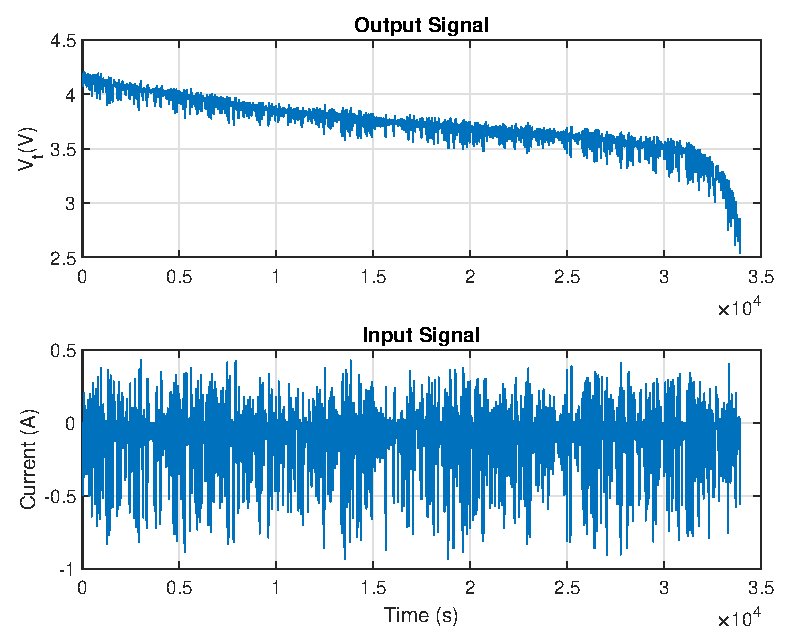
\includegraphics[width=0.85\linewidth]{traindataset}
	\caption{Training dataset}
	\label{fig:traindataset}
\end{figure}

\begin{figure}
	\centering
	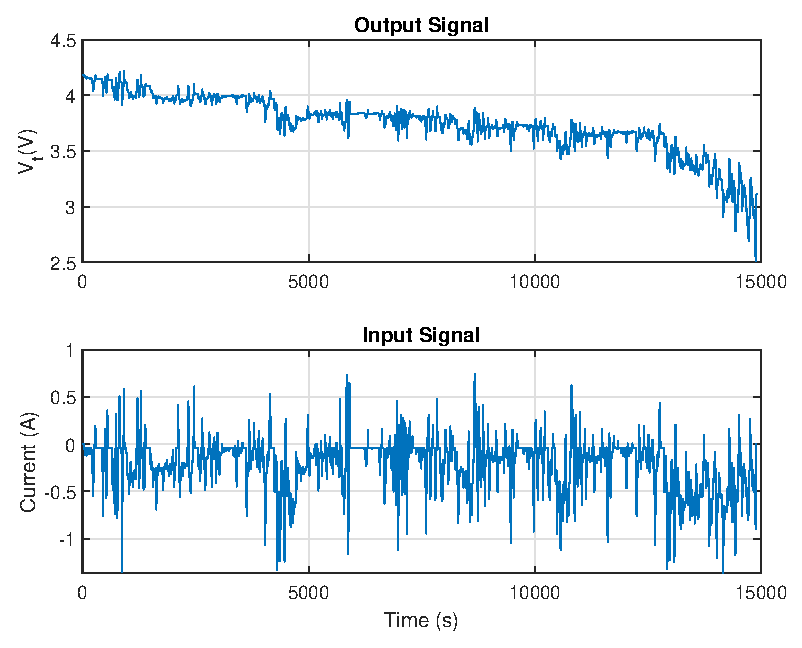
\includegraphics[width=0.85\linewidth]{valdataset}
	\caption{Validation dataset.}
	\label{fig:valdataset}
\end{figure}

\begin{figure}
	\centering
	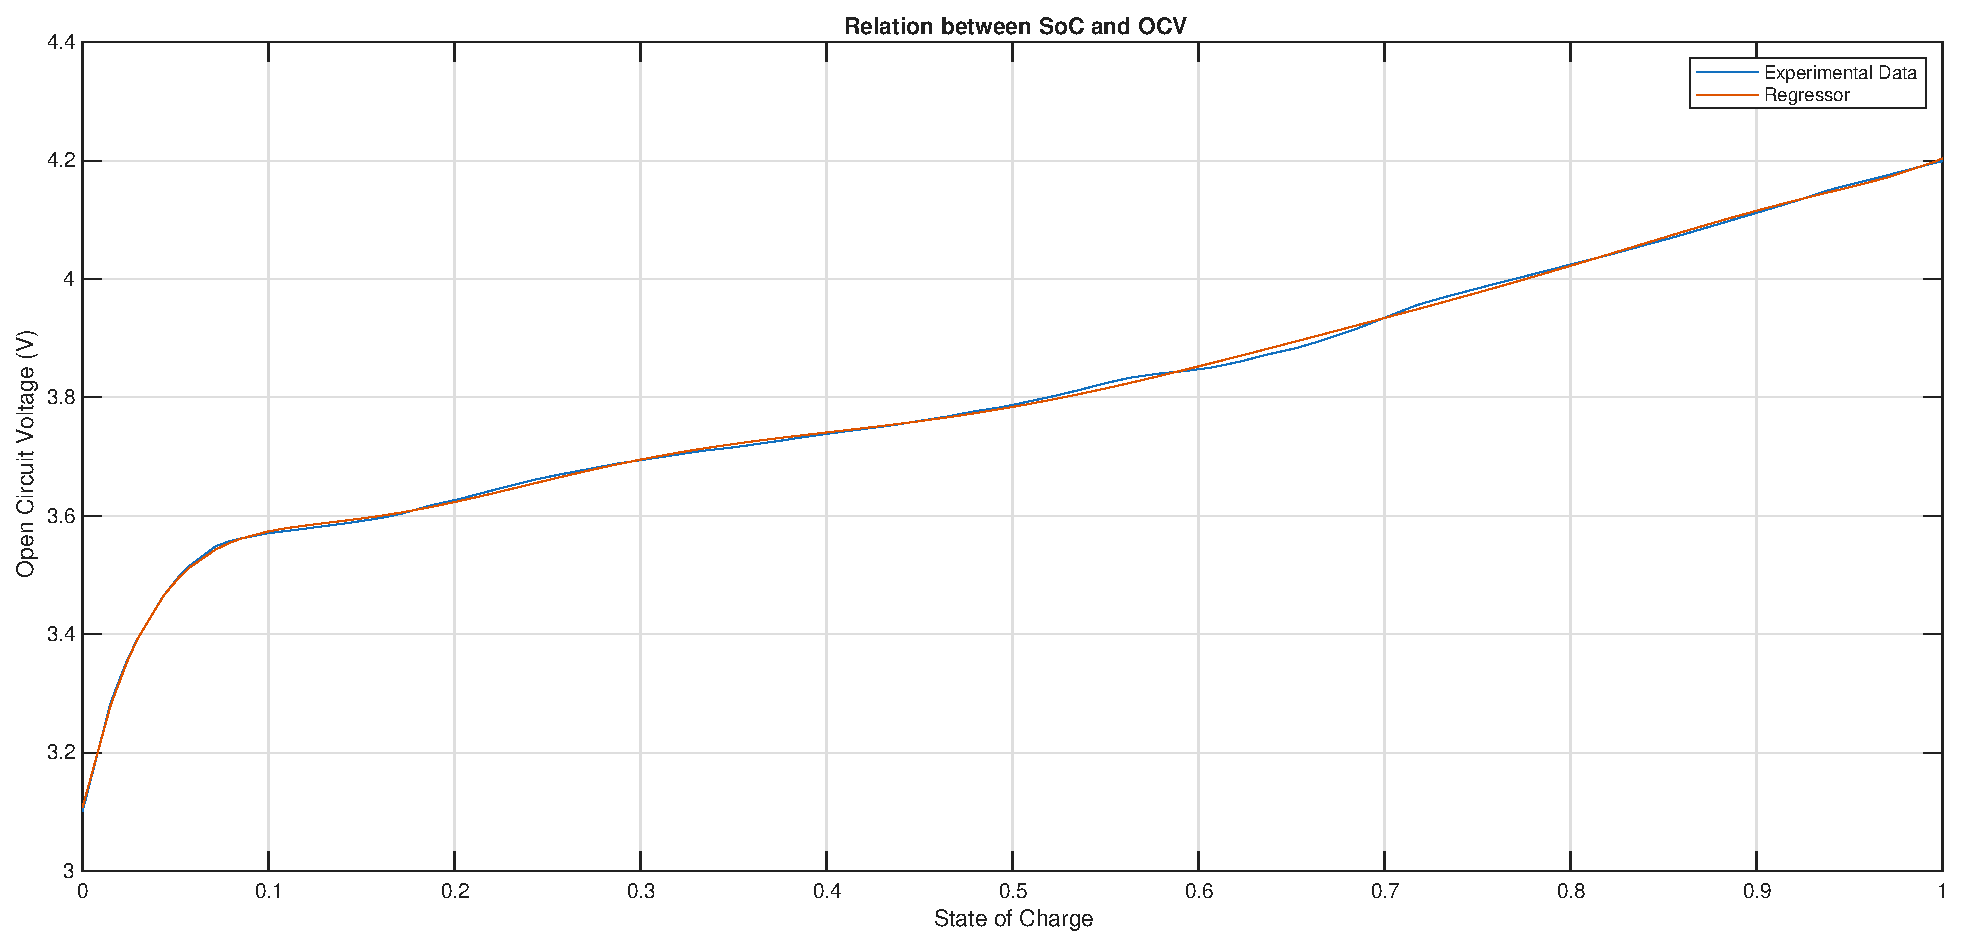
\includegraphics[width=0.7\linewidth]{ocvsoc}
	\caption{Relation between State of Charge and Open Circuit Voltage.}
	\label{fig:ocvsoc}
\end{figure}



\section{Results}

All three ECM models were employed in the construction of the grey-box models, but only the 1RC model was considered in the proposed hybrid approaches that utilize MLP-NN, RBF-NN, and WNN with the specified activation functions. The metrics obtained are exposed in Table \ref{tab:metricstrain} and \ref{tab:metricsval}. The percentage under parenthesis represents the variation of the metric when compared to the 1RC model.

\begin{table}\label{tab:metricstrain}
	\centering
	\caption{Performance metrics of the tuned models and optimization parameters used with the training dataset.}
	\begin{tabular}{c|c|c|c	}
		
		Model& $R^2$ & RMSE (mV) & $N_n$  \\
		\hline
		GB - 1RC & 0.899062 & 75.093275   & \\
		GB - 2RC & 0.902981 & 73.613857  &\\
		GB - PNGV & 0.885879 & 79.843597&\\
		\hline
		GB+MLP - ReLu & 0.994933 ($+10,66\%$) & 16.82379 ($-77.59\%$) & 32 \\
		GB+RBF - GS & 0.996183 ($+10,80\%$)& 16.062378 ($-80.56\%$)& 64 \\
		GB+RBF - IQT & 0.995115 ($+10,68\%$)& 16.492422 ($-78.03\%$) & 32\\
		GB+RBF - TH & 0.996357 ($+10,82\%$)& 14.282856 ($-80.97\%$)& 32 \\
		GB+RBF - TPS & 0.995379 ($+10,71\%$)& 16.062378 ($-78.61\%$) & 64\\
		GB+WNN - Hat & 0.996248 ($+10,81\%$)& 14.456832 ($-80.74\%$) & 64\\
		\hline
	\end{tabular}
\end{table}
\begin{table}\label{tab:metricsval}
	\centering
	\caption{Performance metrics of the tuned models and optimization parameters used with the validation dataset.}
	\begin{tabular}{c|c|c|c	}
		
		Model& $R^2$ & RMSE (mV)& $N_n$  \\
		\hline
		GB - 1RC & 0.337546 & 205.941739   & \\
		GB - 2RC & 0.380221 & 199.198644  &\\
		GB - PNGV & 0.206463 & 225.397426&\\
		\hline
		GB+MLP - ReLu & 0.39147627 ($+15.97\%$) & 197.38199 ($-4.15\%$) & 32 \\
		GB+RBF - GS & 0.399211 ($+18.26\%$) & 196.123456 ($-4.76\%$)& 64 \\
		GB+RBF - IQT & 0.396361 ($+17.42\%$) & 196.585859 ($-4.54\%$)& 32\\
		GB+RBF - TH & 0.392282 ($+16.21\%$)& 197.251235 ($-4.21\%$)& 32 \\
		GB+RBF - TPS & 0.350297 ($+3.77\%$)& 203.951048 ($+0.96\%$)& 64\\
		GB+WNN - Hat & 0.404212 ($+19.75\%$)& 195.305401 ($-5.16\%$)& 64\\
		\hline
	\end{tabular}
\end{table}


The estimated responses for the best grey-box model, and the best hybrid approach are displayed in Figure \ref{fig:2rchyb} .

\begin{figure}
	\centering
	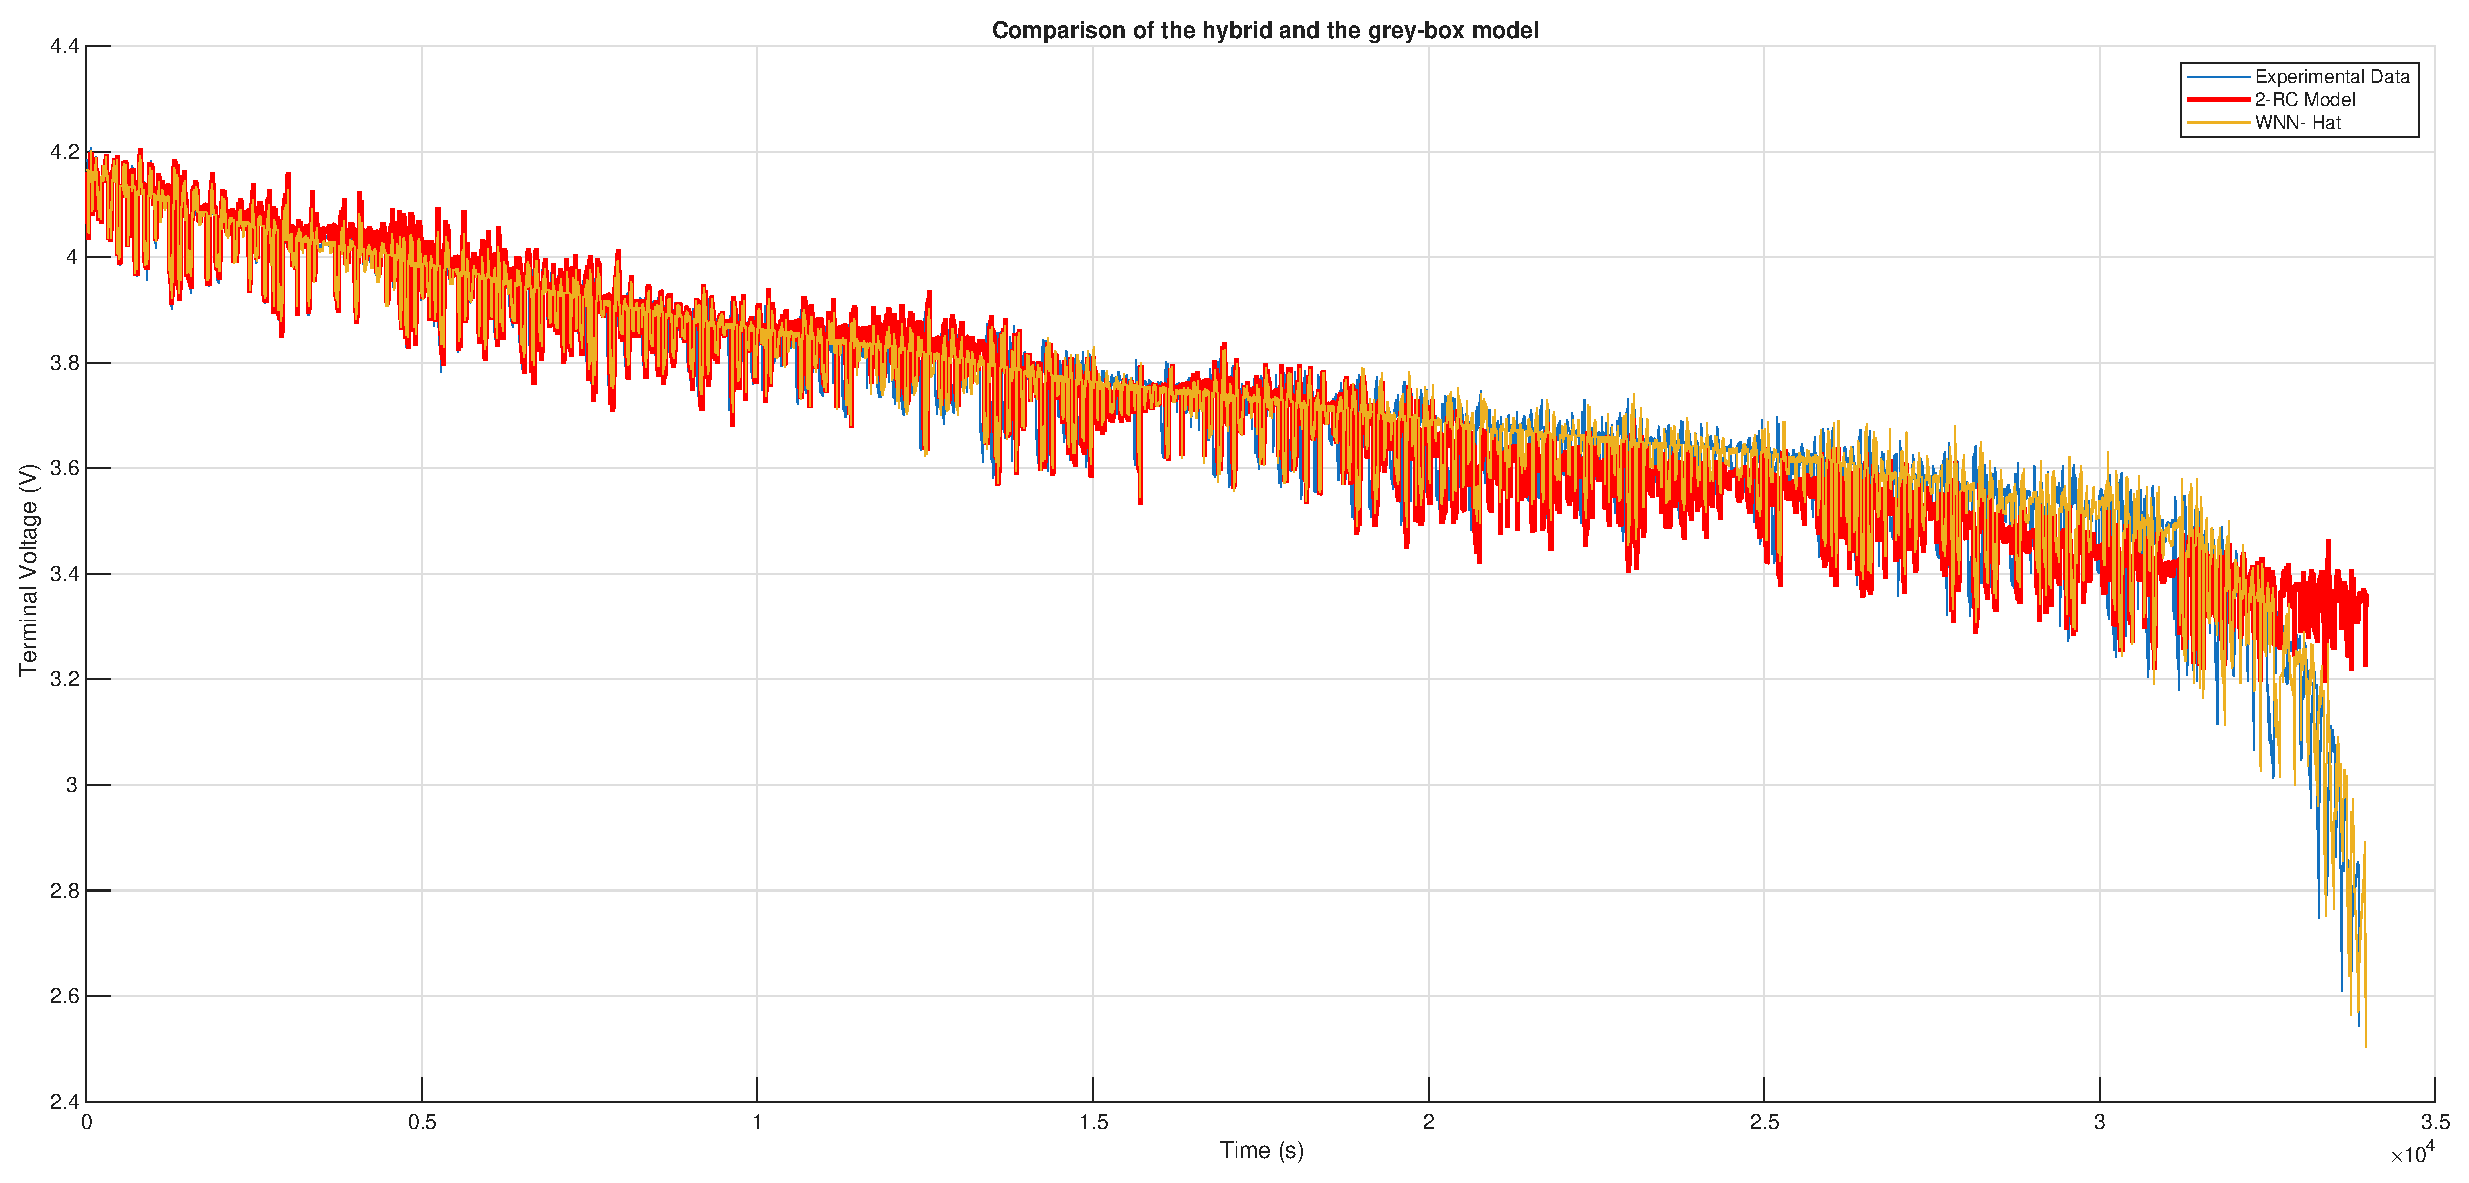
\includegraphics[width=\linewidth]{2rchyb}
	\caption{Output of the 2-RC model, Hybrid model using WNN - Hat and the experimental data.}
	\label{fig:2rchyb}
\end{figure}


Figures \ref{fig:simout} and \ref{fig:simoutval} compares the estimated system responses obtained using the best activation function across the three neural network architectures, along the corresponding residues, with both datasets. Finally, a scatter plot detailing the performance of the best hybrid approach is presented in Figure \ref{fig:scatplot}, and the correlation plots are in Figure \ref{fig:corrtrain} and \ref{fig:corrval}.

\begin{figure}
	\centering
	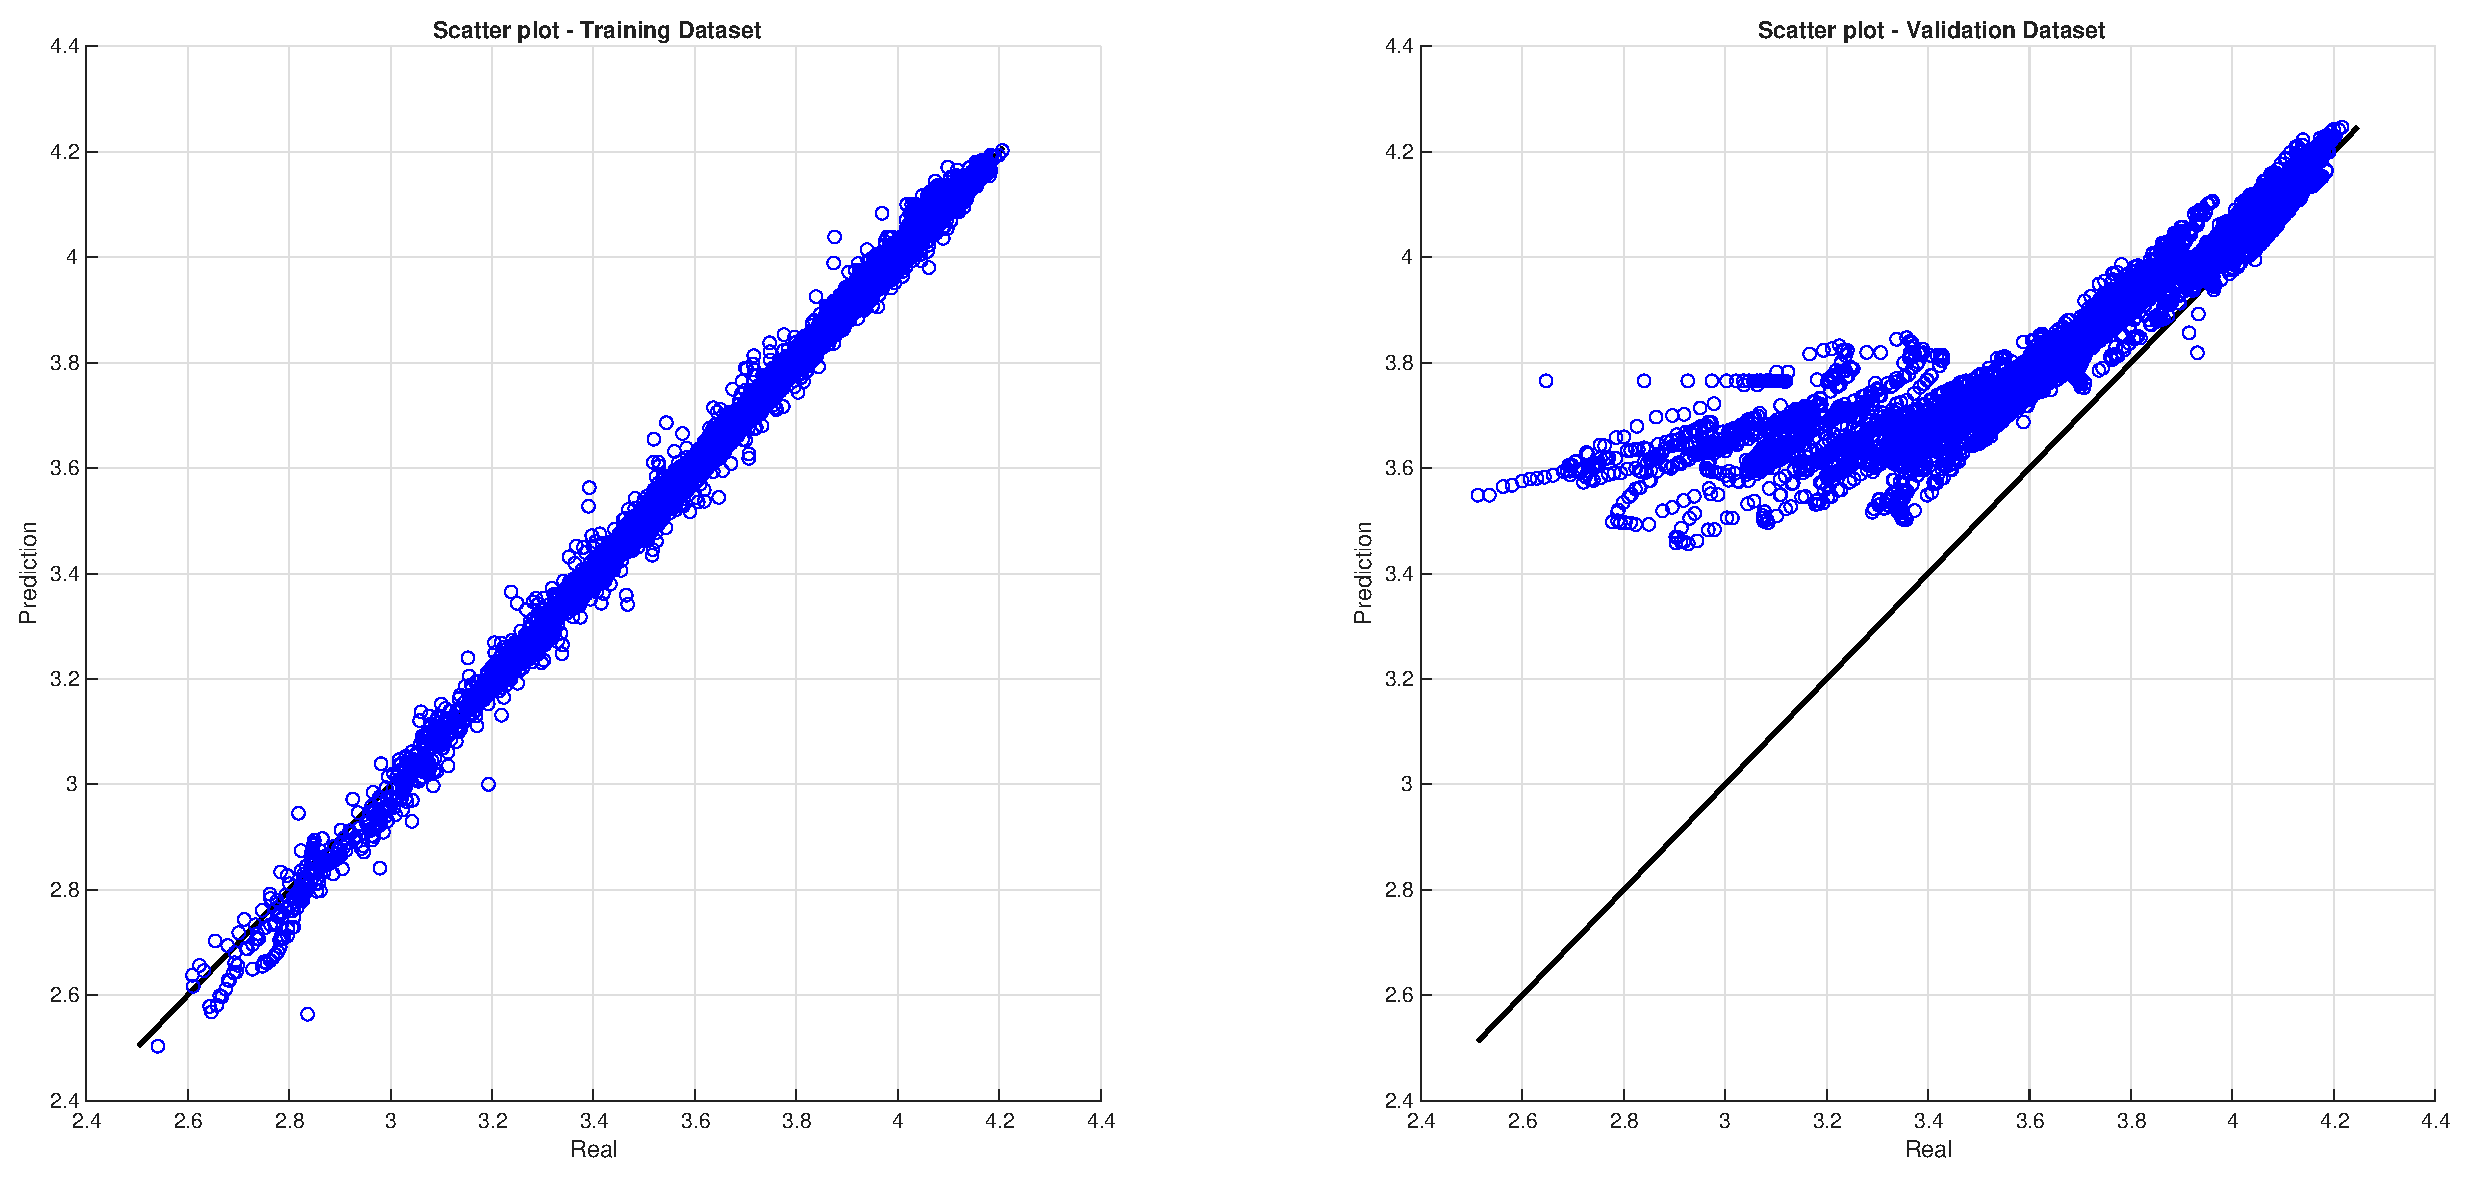
\includegraphics[width=.9\linewidth]{scatplot}
	\caption{Scatter plot of the WNN - Hat Hybrid model.}
	\label{fig:scatplot}
\end{figure}

\begin{figure}
	\centering
	\includegraphics[width=\linewidth]{corrtrain}
	\caption{Correlation tests of WNN - Hat Hybrid model and the training dataset.}
	\label{fig:corrtrain}
\end{figure}

\begin{figure}
	\centering
	\includegraphics[width=\linewidth]{corrval}
	\caption{Correlation tests of WNN - Hat Hybrid model and the validation dataset.}
	\label{fig:corrval}
\end{figure}

\begin{figure*}[ht]
	\centering
	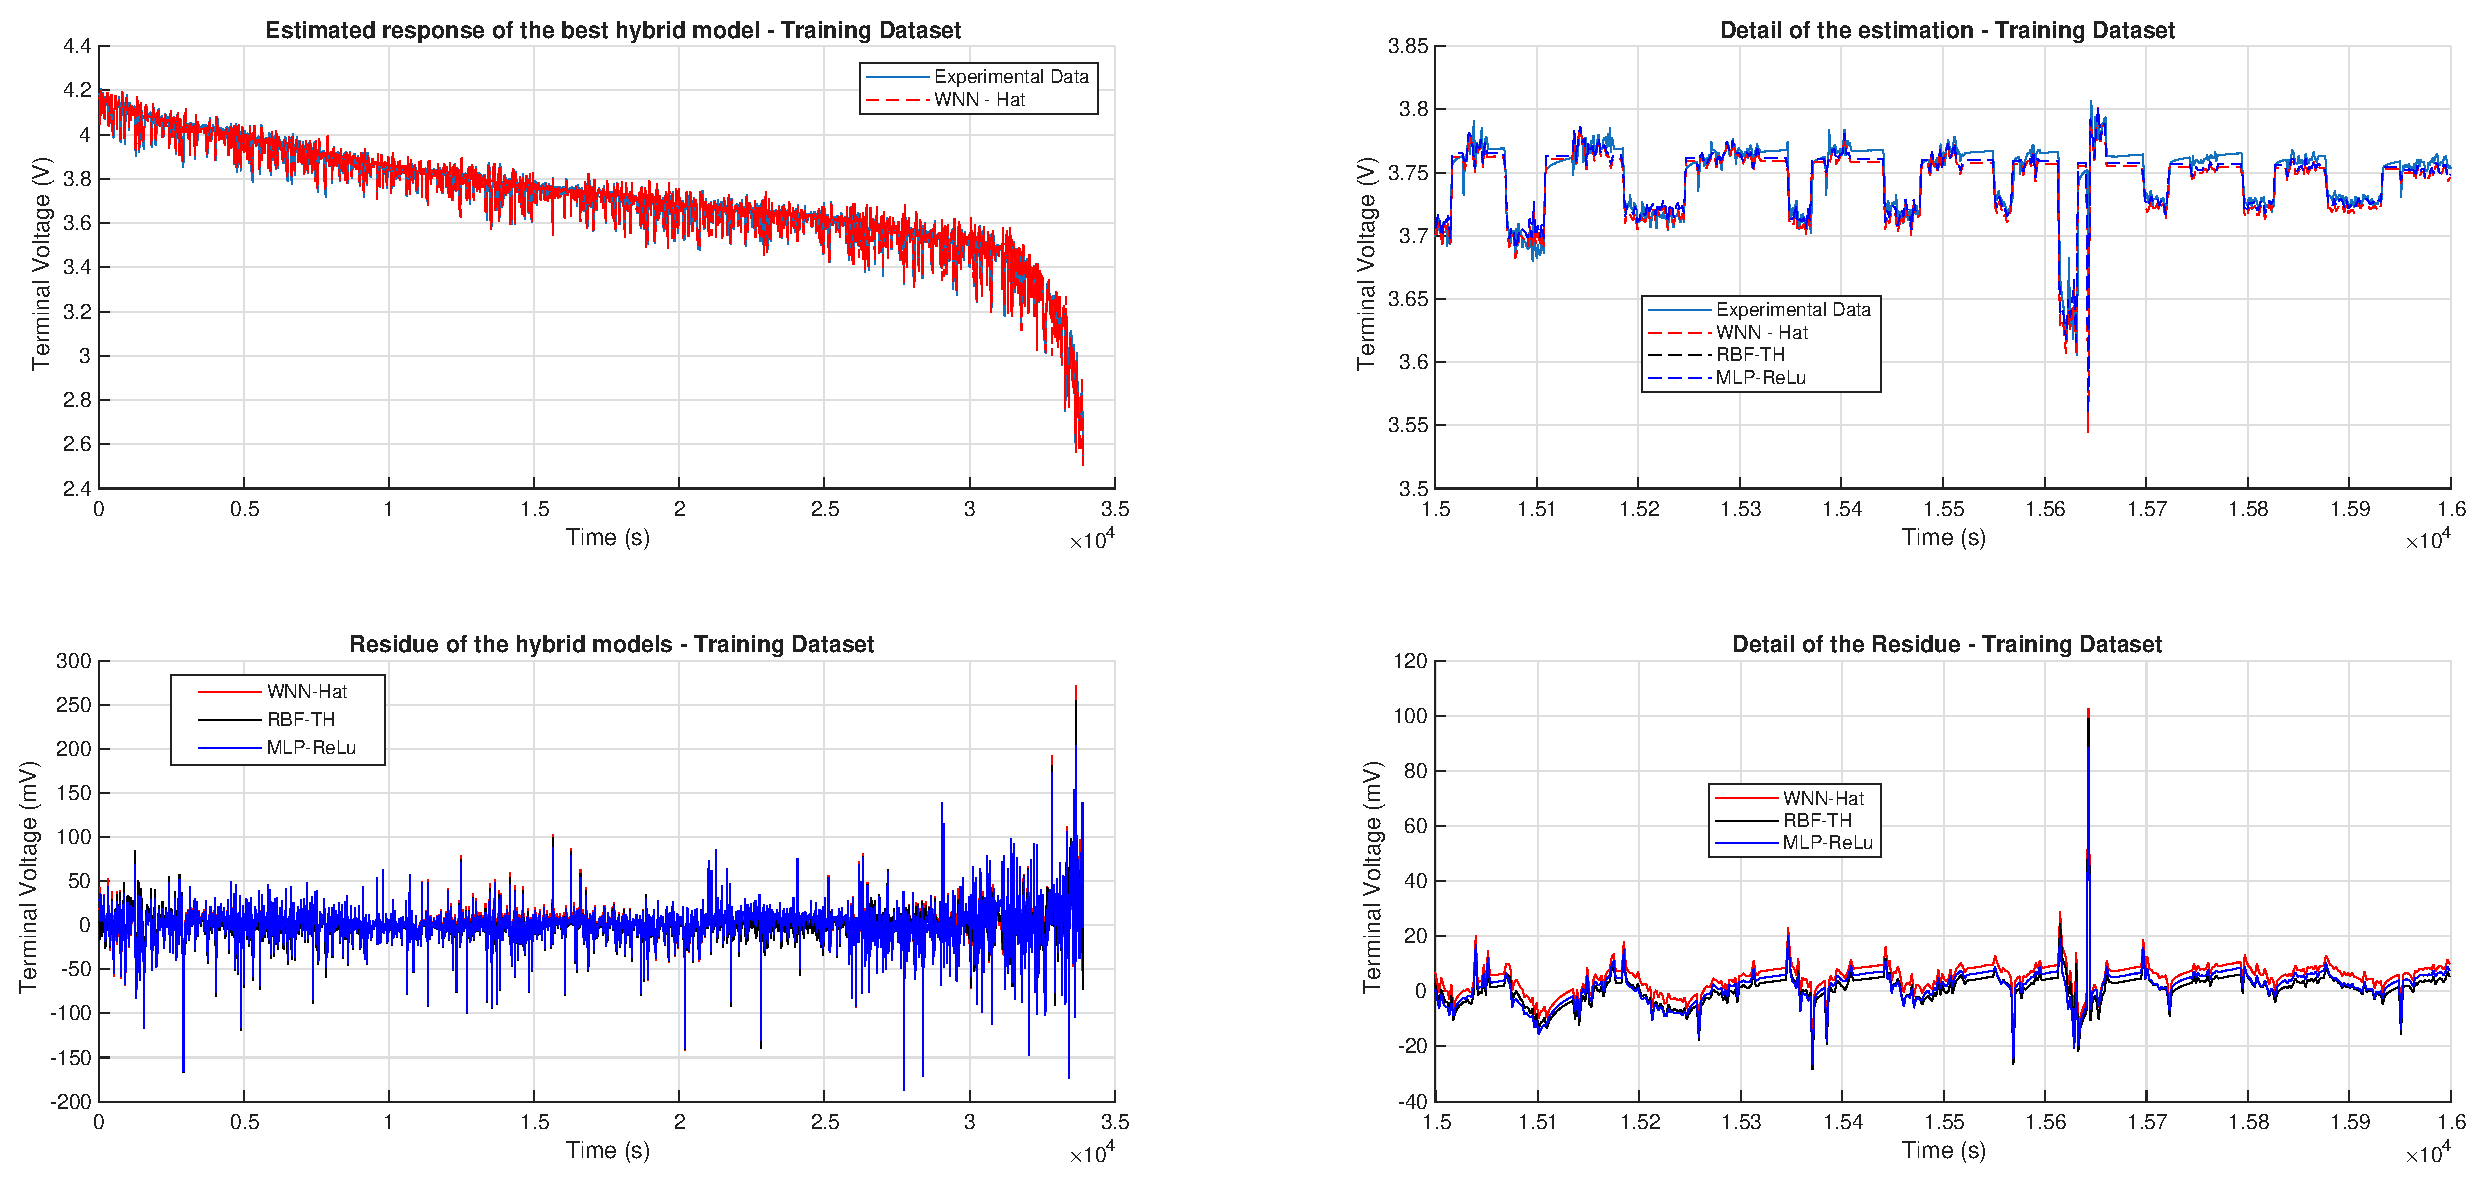
\includegraphics[width=.8\linewidth]{simout}
	\caption{Simulation results of the WNN - Hat Hybrid model compared to the other activation functions with higher performance - Training Dataset.}
	\label{fig:simout}
\end{figure*}

\begin{figure*}[ht]
	\centering
	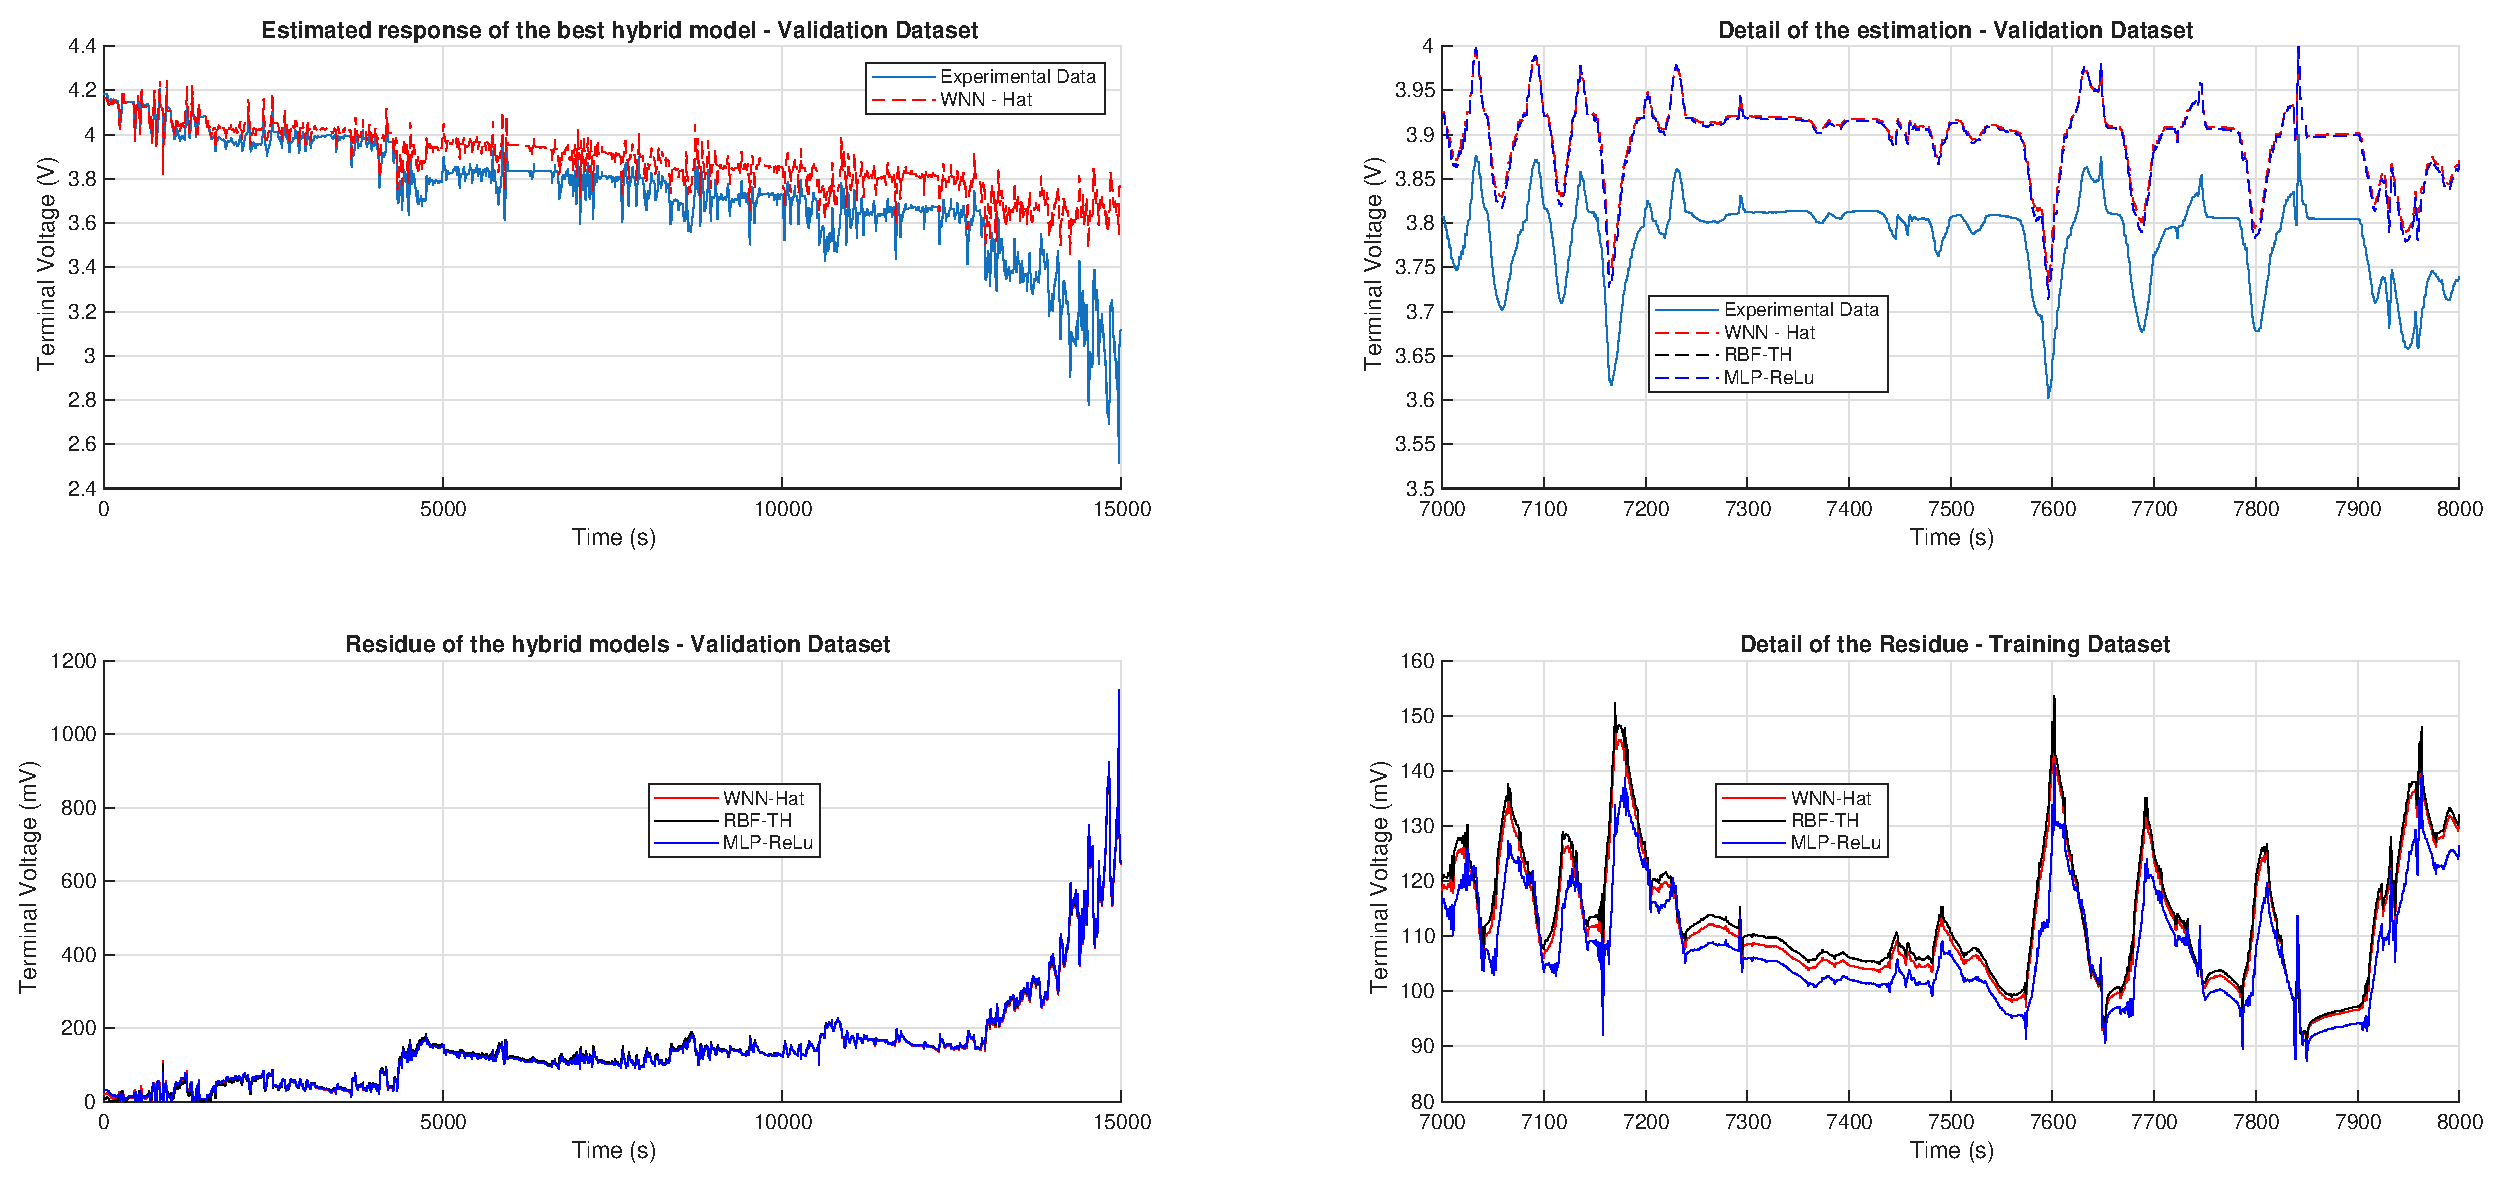
\includegraphics[width=.8\linewidth]{simoutval}
	\caption{Simulation results of the WNN - Hat Hybrid model compared to the other activation functions with higher performance - Validation Dataset.}
	\label{fig:simoutval}
\end{figure*}




\section{Result Analysis}
\section{Results Analysis}

\subsection{Performance of Grey-Box and Hybrid Models}
The initial evaluation of the pure **grey-box Equivalent Circuit Models (ECM)**, namely the IRC, 2RC, and PNGV structures, demonstrated a good level of performance. All three models achieved $\mathbf{R^2}$ values near $\mathbf{90\%}$ on the training dataset. This outcome was close to the expected behavior based on the initial system identification.

However, as the experiment progressed and the battery's **State of Charge (SoC)** varied, the intrinsic Linear Time-Invariant (LTI) assumption of the standard ECMs was violated. This inherent variation causes the fixed model parameters to lose adherence to the experimental data, strongly emphasizing the battery's true **Linear Parameter-Varying (LPV)** nature.

To address this characteristic, the **hybrid models** were introduced, incorporating shallow neural networks to model the non-linear parameter variation as a function of the battery's state. This integration significantly improved the model's fidelity on the training data, with the hybrid architecture achieving $\mathbf{R^2}$ values exceeding $\mathbf{99\%}$ and **Root Mean Square Errors (RMSE)** close to $\mathbf{15\,mV}$. This represents a substantial enhancement over the pure grey-box models, corresponding to an approximate increase of $\mathbf{0.09}$ in $R^2$ and a decrease of about $\mathbf{60\,mV}$ in RMSE (comparing the best hybrid performance against the pure ECM baseline).

\subsection{Evaluation of Neural Network Architectures}
The study investigated various **activation functions** for the **RBF**, **MLP**, and **WNN** architectures. No significant difference in computational complexity was found among the proposed variations. Similarly, the performance metrics (e.g., $R^2$ and RMSE) for all hybrid models were found to differ by less than $\mathbf{0.001}$, confirming that all proposed neural network configurations delivered a satisfactory and comparable performance.

A comparison of the model residues across the hybrid architectures revealed a similar overall behavior. However, the RBF network exhibited a few sporadic peaks in its residue, which accounted for its minor performance difference compared to the MLP and WNN models.

Regarding network complexity, the maximum number of hidden neurons used was $\mathbf{64}$, which resulted in a total of $\mathbf{130}$ parameters for the hybrid model in those cases. This is considered a comparatively small parameter count for a neural network, which is critical for the practical implementation of these models on hardware with limited storage and processing capabilities, especially considering the $\mathbf{2s}$ sampling time of the training data.

\subsection{Generalization and Extrapolation Performance}
The superior performance on the training data is clearly demonstrated in the **scatter plot** (e.g., Figure \ref{fig:scatterplot}), which shows excellent adherence between the WNN model's predictions and the experimental data points.

However, the analysis of the scatter plot for the **validation data** revealed a clear loss of adherence as the terminal voltage and, consequently, the SoC diminished. This degradation is attributed to a significant spectral mismatch between the **input current signal (dynamic profile)** used for validation and the one used for training. This highlights a **generalization failure** where the model struggles to accurately represent the battery's dynamics when exposed to unrepresented, highly dynamic input signals.

Furthermore, a critical limitation observed is the poor performance of the proposed networks during **extrapolation**. If the model is forced to operate at SoC levels or under load conditions outside the boundaries of the training dataset, convergence and accurate prediction cannot be guaranteed, which is a known characteristic of black-box and grey-box data-driven approaches.

\subsection{Correlation Tests and Parameter Estimation}
The **correlation test** results for the training data (Figure \ref{fig:correlation}) show a sharp peak near zero lag. This signifies a near-zero correlation between the model error (residue) and the input signal. This key finding permits the conclusion that the model residue is primarily composed of $\mathbf{random noise}$ and measurement errors, indicating that the model structure itself is robust for the conditions it was trained on. In contrast, the correlation curve for the validation data was noticeably $\mathbf{flatter}$, suggesting that there are potential improvements to be made in the model structure to better capture the battery's dynamics under the unrepresented validation profile.

The estimation of the SoC variation in the ECM is performed using the **Coulomb Counting** method. While this method is essential for its simplicity and computational efficiency, its effectiveness is limited by its sensitivity to the initial SoC value and current measurement noise, which leads to **integration drift** over long periods. In this framework, the estimation accuracy relies on the overall performance of the full state-space system, which must eventually be integrated with a state observer (like an EKF) to correct the SoC estimate based on the terminal voltage measurements.

\subsection{Comparison with Related Work}
The experimental data used in this work was derived from the same source as the study presented by **Sheikh et al. (2024)**, who also investigated LPV battery modeling but utilized a different identification technique based on sparse regression in the input-output representation. Comparing the results, Sheikh et al. (2024) reported an $\mathbf{RMSE \approx 24.5 mV}$ for their best-performing LPV model under drive-cycle validation. The hybrid grey-box models proposed here achieved a lower RMSE of $\mathbf{15 mV}$ on the training set and demonstrated superior fidelity within the trained operating range. Both studies collectively reinforce the concept of the battery ECM as an **LPV system** and underscore the necessity of parameter scheduling based on operating conditions like SoC.

\section{Conclusion}

This work successfully ratified the importance of the Equivalent Circuit Model (ECM) as a pragmatic and efficient standard for Battery Management Systems (BMS). It confirmed the LPV (Linear Parameter-Varying) nature of the battery's dynamics, highlighting the challenge of maintaining model accuracy as operating conditions vary. The main difficulty encountered was the generalization failure of the models when exposed to dynamic load profiles outside the domain of the training data.

The principal results demonstrated that the hybrid grey-box framework, which utilizes shallow neural networks for parameter scheduling, significantly enhances the model's accuracy on the training data, yielding $\mathbf{R^2 > 99\%}$ and an $\mathbf{RMSE \approx 15 mV}$. This performance constitutes a notable improvement over pure grey-box models and surpasses the $\mathbf{RMSE \approx 24.5 mV}$ reported \cite{Sheikh2024}, who employed the same underlying data source. The network complexity was also found to be low, with a maximum of $\mathbf{130}$ parameters, making the model suitable for embedded applications.

For future work, we suggest the online implementation of the hybrid model using an adaptive training algorithm for the neural networks. This would allow the model to continuously learn and adapt to real-time variations in charging/discharging conditions and aging effects, thereby mitigating the generalization issues observed with the current off-line identified model. Further research should also focus on integrating the identified hybrid model into a state estimation framework, such as an Extended Kalman Filter (EKF), for robust, real-time tracking of State of Charge (SoC) and State of Health (SoH).

\bibliographystyle{ieeetr}
\bibliography{export.bib}
\end{document}	

